\documentclass[11pt,a4paper]{article}
% === Packages ===
\usepackage[utf8]{inputenc}
\usepackage[T1]{fontenc}
\usepackage{mathpazo}           % Palatino font (common in bioRxiv preprints)
\usepackage[margin=2.5cm]{geometry}
\usepackage{graphicx}
\usepackage{booktabs}
\usepackage{hyperref}
\usepackage{xcolor}
\usepackage{amsmath}
\usepackage{authblk}
\usepackage{lineno}             % Line numbers (required for bioRxiv)
\usepackage{setspace}
\usepackage{natbib}
\usepackage{caption}
\usepackage{float}
% === Hyperref setup ===
\hypersetup{
    colorlinks=true,
    linkcolor=blue!70!black,
    citecolor=blue!70!black,
    urlcolor=blue!70!black
}
% === Line numbers ===
\linenumbers
% === Spacing ===
\onehalfspacing
% === Custom commands ===
\newcommand{\betat}{\ensuremath{\beta}}
% === Title ===
\title{\Large\textbf{Spectral Exponents of the Twelve-Lead ECG Reveal the Anatomy of Cardiac Conduction Disorders and a Bifurcation Between Aging and Disease}}
% === Authors ===
\author[1]{Theodor Spiro}
% === Affiliations ===
\affil[1]{Independent Researcher, Paris, France}
% === Date ===
\date{\today}
\begin{document}
\maketitle
% === Correspondence ===
\noindent\textbf{Correspondence:} theospirin@gmail.com\\
\noindent\textbf{ORCID:} \url{https://orcid.org/0009-0004-5382-9346}
\vspace{1em}
\hrule
\vspace{1em}
% ================================================================
% ABSTRACT
% ================================================================
\begin{abstract}
\noindent
The aperiodic ($1/f^\beta$) component of the electrocardiogram carries information about broadband cardiac electrical dynamics, yet it remains largely unexplored as a quantitative marker of conduction system integrity. Here we apply Irregular-Resampling Auto-Spectral Analysis (IRASA) to 412,730 twelve-lead ECG recordings across three datasets spanning three continents---PTB-XL (Germany, $n = 21{,}799$), Chapman-Shaoxing (China, $n = 45{,}152$), and CODE-15\% (Brazil, $n = 345{,}779$)---to extract the spectral exponent $\beta$, a single number per lead quantifying the balance between order and disorder in the cardiac electrical signal.
We report five findings. First, each diagnostic category deviates from the healthy reference in a specific direction and magnitude, with conduction disturbances showing the strongest divergence (Cohen's $d = 0.99$). Second, the twelve-lead $\beta$-vector encodes the spatial anatomy of the conduction system: a classifier distinguishes complete left from complete right bundle branch block with AUC $= 0.982$ on the discovery cohort (PTB-XL), and this result replicates exactly on two independent external cohorts (AUC $= 0.982$ on Chapman-Shaoxing; AUC $= 0.979$ on CODE-15\%), despite substantial variation in absolute $\beta$-values across recording equipment ($\beta_\text{NORM} = 1.52$--$2.75$). Third, within a curated healthy cohort (PTB-XL), aging and pathology drive $\beta$ in opposite directions---healthy aging flattens the spectrum ($\beta$ decreases, $\rho = -0.179$) while overt conduction disease steepens it ($\beta$ increases), creating a bifurcation from the healthy operating point. Beat-to-beat morphological variability independently confirms age-related complexity loss ($\rho = 0.165$, $p < 10^{-19}$). Fourth, among ECGs labeled normal by cardiologists, $\beta$ distinguishes truly clean recordings from those with subclinical conduction findings (AUC $= 0.754$), with the direction of $\beta$-shift inverted relative to overt disease. Fifth, $\beta$ does not independently predict all-cause mortality beyond established diagnoses (adjusted HR $= 1.02$, $p = 0.83$ in CODE-15\%), establishing it as a diagnostic marker of conduction anatomy rather than an independent prognostic biomarker.
These results demonstrate that the spectral exponent captures a cross-population invariant of cardiac electrophysiology: the geometry of the twelve-lead $\beta$-vector is determined by conduction system anatomy and is reproducible across equipment, ethnicity, and geography.
\vspace{0.5em}
\noindent\textbf{Keywords:} electrocardiography, spectral exponent, 1/$f$ noise, IRASA, cardiac conduction, aging, PTB-XL, external validation, cross-population invariance
\end{abstract}
\newpage
% ================================================================
% 1. INTRODUCTION
% ================================================================
\section{Introduction}
The electrocardiogram (ECG) has been the primary tool for cardiac diagnosis for over a century. Clinical interpretation focuses on periodic features---heart rate, P-wave morphology, QRS duration, ST-segment deviation, QT interval---that reflect specific phases of the cardiac cycle. Deep learning approaches have extended this further, achieving diagnostic performance exceeding that of expert cardiologists by extracting complex morphological patterns from the full waveform \citep{Strodthoff2021, Ribeiro2020}.
Yet the ECG signal also contains an aperiodic component: a broadband $1/f^\beta$ background upon which periodic cardiac oscillations are superimposed. This aperiodic component, characterized by the spectral exponent $\beta$, reflects the statistical structure of electrical fluctuations across all frequencies simultaneously. In neurophysiology, the analogous parameter in EEG/MEG signals has been extensively studied and linked to excitation-inhibition balance \citep{Gao2017}, arousal \citep{Lendner2020}, and aging \citep{Voytek2015}. In cardiology, however, the focus has been almost exclusively on heart rate variability (HRV)---the $1/f$ scaling of beat-to-beat interval fluctuations---rather than on the spectral properties of the ECG waveform itself.
The HRV literature has established that healthy cardiac dynamics exhibit complex, multiscale fluctuations near a critical state, while aging and disease degrade this complexity \citep{Goldberger2002}. Detrended fluctuation analysis of RR-interval series reveals that healthy hearts show scaling exponents near $\alpha \approx 1.0$ (equivalent to $1/f$ noise), with systematic deviations in heart failure, atrial fibrillation, and aging \citep{Peng1995, Ivanov1999}. \citet{Lipsitz1992} formalized this as the ``loss of complexity'' hypothesis: healthy physiology is characterized by complex, multiscale dynamics, while disease and aging produce a degradation toward either excessive regularity or uncorrelated randomness.
Whether the same principles apply to the ECG waveform---the voltage signal itself, not the derived RR-interval series---remains largely untested. The ECG waveform reflects the collective depolarization and repolarization of approximately two billion cardiomyocytes, and its spectral properties are determined by the quality of electrical coupling (gap junctions), conduction velocity (ion channels), and tissue architecture (fibrosis, scarring). A handful of studies have applied multifractal analysis to ECG voltage signals \citep{Yang2020, Shekatkar2017} or examined ECG spectral slopes in the context of aging \citep{Schmidt2025}, but no systematic analysis has mapped the spectral exponent across diagnostic categories in a large clinical dataset.
A key methodological challenge is that the ECG contains powerful periodic components---QRS harmonics extending to the 15th harmonic of heart rate---that contaminate spectral slope estimation if not properly separated. \citet{Schmidt2025} identified a spectral knee near 15~Hz and employed IRASA (Irregular-Resampling Auto-Spectral Analysis; \citealt{Wen2016}) to separate periodic and aperiodic components. We adopt the same approach on a substantially larger dataset with clinical diagnostic labels.
Here we analyze the PTB-XL dataset \citep{Wagner2020}---21,799 ten-second, twelve-lead ECG recordings from 18,869 patients with expert diagnostic labels spanning five superclasses and 23 subclasses---and externally validate on two independent datasets totaling over 390,000 additional recordings. We extract the spectral exponent $\beta$ from the aperiodic component of each lead using IRASA and investigate five questions: (1)~Does $\beta$ differ systematically across diagnostic categories? (2)~Can the twelve-lead $\beta$-vector discriminate conduction disorder subtypes and reconstruct lesion anatomy? (3)~How does $\beta$ change with healthy aging, and how does this relate to disease-related changes? (4)~Can $\beta$ detect subclinical conduction abnormalities in recordings labeled normal? (5)~Does $\beta$ independently predict mortality?
% ================================================================
% 2. METHODS
% ================================================================
\section{Methods}
\subsection{Discovery Dataset}
We used the PTB-XL electrocardiography dataset \citep{Wagner2020}, version 1.0.3, accessed via PhysioNet and Kaggle. The dataset contains 21,799 ten-second, twelve-lead ECG recordings sampled at 500~Hz from 18,869 unique patients (52\% male, median age 62 years, range 2--89; one outlier with age $= 300$ excluded). Each recording was independently annotated by up to two cardiologists with diagnostic labels organized into five superclasses: Normal (NORM, $n = 9{,}514$), Myocardial Infarction (MI, $n = 5{,}469$), ST/T Changes (STTC, $n = 5{,}235$), Conduction Disturbance (CD, $n = 4{,}898$), and Hypertrophy (HYP, $n = 2{,}649$). Recordings may carry multiple labels. Within CD, subclasses include Complete Left Bundle Branch Block (CLBBB, $n = 536$), Complete Right Bundle Branch Block (CRBBB, $n = 537$), Incomplete Right Bundle Branch Block (IRBBB, $n = 1{,}102$), Left Anterior Fascicular Block (LAFB, $n = 1{,}604$), First-Degree AV Block (1AVB, $n = 779$), and Intraventricular Conduction Delay (IVCD, $n = 780$). Subclass counts reflect recordings with $\geq 80\%$ annotator confidence. We used the predefined stratified folds for train-test splits, with folds 9--10 reserved for testing.
\subsection{Signal Preprocessing}
Each twelve-lead ECG was preprocessed as follows: (1)~bandpass filtering at 0.5--100~Hz (4th-order Butterworth) to remove baseline drift and high-frequency noise; (2)~notch filtering at 50~Hz (2nd-order IIR) to remove powerline interference.
\subsection{Spectral Exponent Extraction via IRASA}
We extracted the aperiodic spectral exponent $\beta$ using IRASA \citep{Wen2016}. IRASA exploits the fact that resampling a signal at an irrational rate $h$ shifts periodic (oscillatory) components in the frequency domain but preserves the power-law structure of the aperiodic component. By computing the power spectral density (PSD) at multiple resampling factors ($h = 1.1, 1.15, \ldots, 1.9$) and taking the geometric mean of each $(h, 1/h)$ pair, oscillatory peaks are attenuated while the aperiodic background is preserved.
For each lead of each recording, we: (1)~computed the PSD using Welch's method (2-second Hanning windows, 50\% overlap); (2)~applied IRASA with 17 resampling factors to obtain the fractal (aperiodic) PSD; (3)~performed linear regression of $\log_{10}(\text{Power})$ on $\log_{10}(\text{Frequency})$ in the range 2--45~Hz to obtain the spectral exponent $\beta$ and the coefficient of determination $R^2$.
This procedure yields, for each recording, a 12-dimensional $\beta$-vector $[\beta_\text{I}, \beta_\text{II}, \ldots, \beta_\text{V6}]$ and a corresponding $R^2$-vector.
\subsection{Derived Metrics}
From the 12-dimensional $\beta$-vector, we computed: $\beta_\text{mean}$ (mean across all 12 leads), $\sigma_\beta$ (standard deviation across leads), regional means ($\beta_\text{anterior}$ for V1--V4, $\beta_\text{lateral}$ for I, aVL, V5, V6, $\beta_\text{inferior}$ for II, III, aVF), and beat-to-beat morphological variability (defined as $1 - \text{mean correlation of individual beats with the average template}$).
\subsection{Statistical Analysis}
Group comparisons used the Kruskal-Wallis test with post-hoc Mann-Whitney U tests and Bonferroni correction. Effect sizes are reported as Cohen's $d$. Age-related trends were assessed by Spearman correlation and segmented regression with breakpoint estimation (Davies test). ANCOVA with age, sex, and recording device as covariates confirmed diagnostic effects.
\subsection{Classification}
We used logistic regression, random forest (500 trees), and gradient boosting machine (GBM, 200 trees) with features consisting of per-lead $\beta$ and $R^2$ values (24 features), regional means and $\sigma_\beta$ (6 features), and demographics (age, sex). Performance was evaluated by AUC-ROC on held-out test folds.
\subsection{External Validation Datasets}
\textbf{Chapman-Shaoxing} \citep{Zheng2020}: 45,152 twelve-lead ECGs at 500~Hz from Shaoxing People's Hospital, China (GE MUSE system). Labels include CLBBB ($n = 213$) and CRBBB ($n = 1{,}096$).
\textbf{CODE-15\%} \citep{Ribeiro2020}: 345,779 twelve-lead ECGs at 400~Hz from the Telehealth Network of Minas Gerais, Brazil. Labels include LBBB ($n = 414$) and RBBB ($n = 557$). Mortality follow-up data available. IRASA frequency range adjusted to 2--40~Hz.
For both external datasets, preprocessing and $\beta$-extraction were identical to PTB-XL except that CODE-15\% used a 60~Hz notch filter (Brazilian powerline standard). The lower sampling rate of CODE-15\% (400~Hz vs.\ 500~Hz) reduces the Nyquist frequency from 250 to 200~Hz, but our fitting range (2--40~Hz for CODE-15\%, 2--45~Hz for 500~Hz datasets) lies well within the resolved bandwidth. The spectral exponent $\beta$ is extracted from the aperiodic component in this low-frequency range and is not affected by the difference in Nyquist frequency.
\subsection{Subclinical Conduction Findings}
To test whether $\beta$ detects subclinical conduction abnormalities, we identified recordings labeled NORM ($\geq 80\%$ confidence) that also carried low-confidence annotations for conduction-related codes. Specifically, we defined ``subclinical'' as any NORM recording co-annotated with one or more of: IRBBB ($n = 209$), IVCD ($n = 80$), 1AVB ($n = 23$), LAFB ($n = 14$), or LPFB ($n = 6$), totaling 328 recordings. The ``pure NORM'' control group consisted of 179 recordings with NORM as the sole annotation.
\subsection{Mortality Analysis}
In CODE-15\%, we assessed whether $\beta$ independently predicts all-cause mortality using Cox proportional hazards regression at three levels of adjustment: (1)~unadjusted; (2)~age and sex; (3)~age, sex, and all diagnostic labels.
% ================================================================
% 3. RESULTS
% ================================================================
\section{Results}
\subsection{The $\beta$-Landscape of Cardiac Diagnoses}
The healthy heart operates at a characteristic spectral exponent $\beta_\text{mean} = 1.76 \pm 0.34$. Each diagnostic superclass shows a distinct $\beta$-profile (Kruskal-Wallis $H = 649$, $p < 10^{-139}$; Figure~\ref{fig:landscape}a). Conduction Disturbance (CD) is the strongest outlier, with $\beta_\text{mean} = 2.15 \pm 0.63$ (Cohen's $d = 0.99$ vs.\ NORM, $p < 10^{-124}$). Myocardial Infarction (MI, $d = 0.28$) and Hypertrophy (HYP, $d = 0.29$) show moderate elevations. ST/T Changes do not differ significantly from NORM ($d = 0.02$), consistent with STTC reflecting repolarization rather than conduction abnormalities.
ANCOVA confirmed that the diagnostic effect is not confounded by demographics: $F = 333$, $p < 10^{-276}$, partial $\eta^2 = 0.076$.
The twelve-lead $\beta$-vector reveals spatial specificity (Figure~\ref{fig:landscape}c). CLBBB produces extreme $\beta$-elevation in V1--V4 ($\Delta\beta$ up to $+1.47$ in V3), corresponding to the anatomical course of the left bundle branch through the interventricular septum. CRBBB shows moderate elevation primarily in V1 ($\Delta\beta = +0.49$).

\begin{figure}[H]
\centering
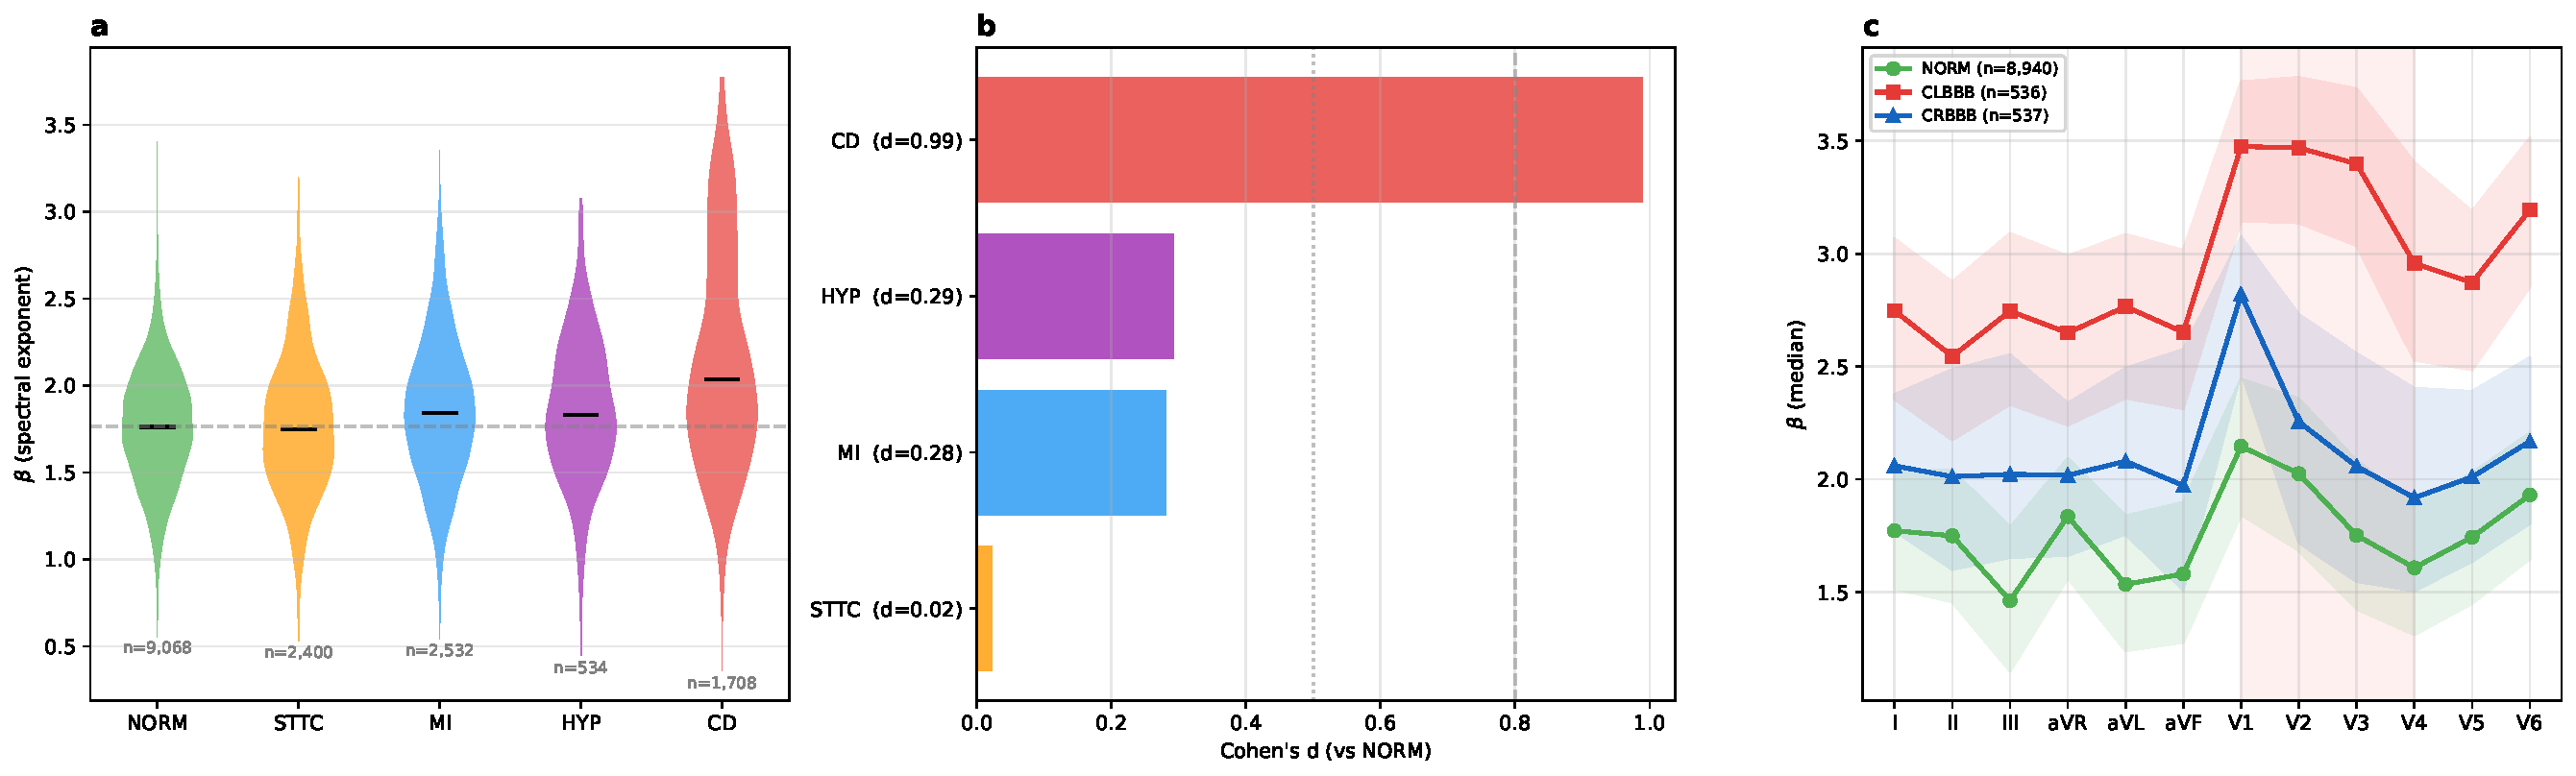
\includegraphics[width=\textwidth]{figures/fig1_beta_landscape.pdf}
\caption{\textbf{The $\beta$-landscape of cardiac diagnoses.} (a)~Violin plots of $\beta_\text{mean}$ for each diagnostic superclass. Horizontal dashed line marks $\beta = 1.76$. CD is the strongest outlier (Cohen's $d = 0.99$). (b)~Cohen's $d$ effect sizes vs.\ NORM. (c)~Spatial fingerprint: median $\beta$ per lead for NORM, CLBBB, and CRBBB. Shaded region marks precordial leads V1--V4.}
\label{fig:landscape}
\end{figure}

\subsection{Spectral Anatomy of Conduction Disorder Subtypes}
A multiclass classifier distinguishing six CD subtypes achieved macro-averaged AUC $= 0.862$ (Figure~\ref{fig:anatomy}b). Per-subtype AUCs ranged from 0.974 (CLBBB) to 0.774 (IVCD).
The pairwise CLBBB vs.\ CRBBB classification achieved AUC $= 0.982$ (Figure~\ref{fig:anatomy}c). For context, deep learning on raw waveforms achieves AUC $\approx 0.99$ using $\sim$60,000 input features \citep{Strodthoff2021}. Our approach reaches 98.2\% of that performance with 54 interpretable features.
Radar plots of $\Delta\beta$ per lead for each subtype (Figure~\ref{fig:anatomy}e) directly map lesion anatomy: CLBBB shows dominant elevation in V1--V4 (left bundle through the septum); CRBBB shows focal elevation in V1 (right bundle proximity); LAFB shows elevation centered on aVL (anterior fascicle to lateral wall); 1AVB shows minimal spatial signature (AV-node pathology produces diffuse delay).
Feature importance analysis confirms anatomical specificity: $R^2$ in V1 is the single most important feature (importance $= 0.298$).

\begin{figure}[H]
\centering
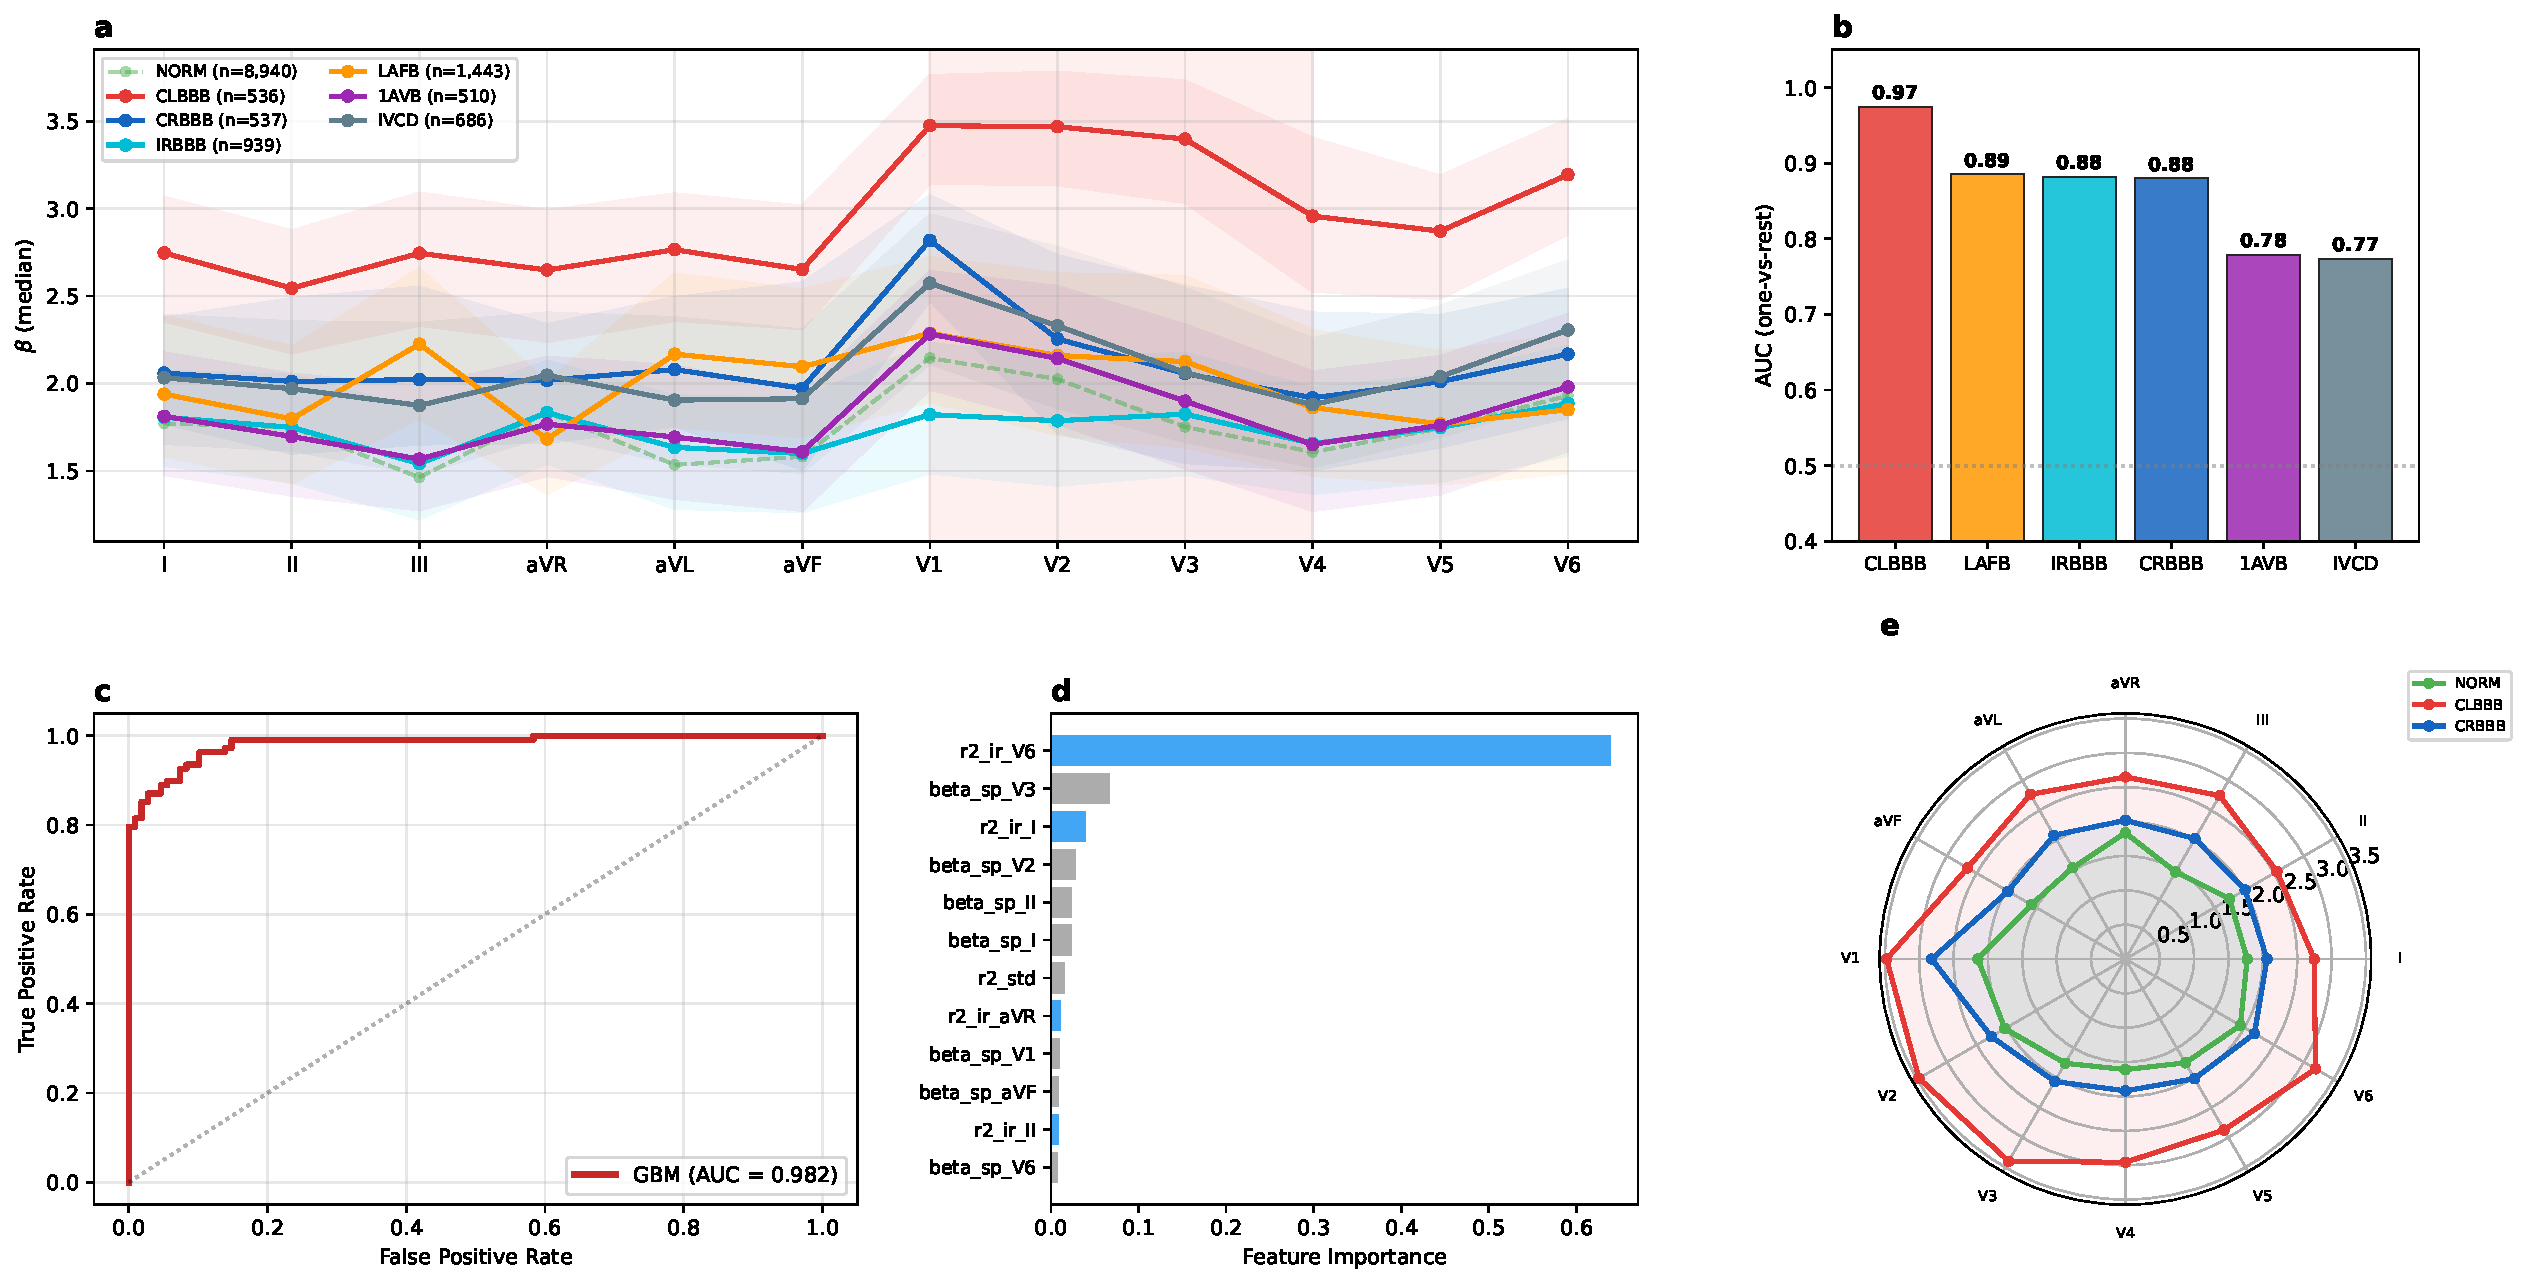
\includegraphics[width=\textwidth]{figures/fig2_spectral_anatomy.pdf}
\caption{\textbf{Spectral anatomy of conduction disorder subtypes.} (a)~Spatial fingerprints of six CD subtypes. (b)~Per-subtype AUC (one-vs-rest). (c)~ROC for CLBBB vs.\ CRBBB (AUC $= 0.982$). (d)~Feature importance for CLBBB vs.\ CRBBB classifier. (e)~Radar plot of $\beta$ per lead.}
\label{fig:anatomy}
\end{figure}

\subsection{Aging Bifurcation: Opposite Trajectories of Age and Disease}
Among 8,940 NORM recordings, $\beta_\text{mean}$ declines with age (Spearman $\rho = -0.179$, $p < 10^{-65}$; Figure~\ref{fig:aging}a). Women show higher baseline $\beta$ but steeper decline ($\rho_F = -0.22$ vs.\ $\rho_M = -0.14$).
This direction is opposite to overt pathology: CD and MI shift $\beta$ \textit{upward}, while aging shifts $\beta$ \textit{downward} (Figure~\ref{fig:aging}c). The healthy operating point sits at a bifurcation between two modes of complexity loss: (1)~aging-related spectral flattening (micro-fragmentation of conduction) and (2)~disease-related spectral steepening (large-scale conduction block).
Segmented regression identifies a breakpoint at age 53 ($F = 17.8$, $p = 1.9 \times 10^{-8}$; Figure~\ref{fig:aging}b), after which spatial heterogeneity ($\sigma_\beta$) accelerates. Beat-to-beat morphological variability independently increases with age ($\rho = 0.165$, $p < 10^{-19}$).

\begin{figure}[H]
\centering
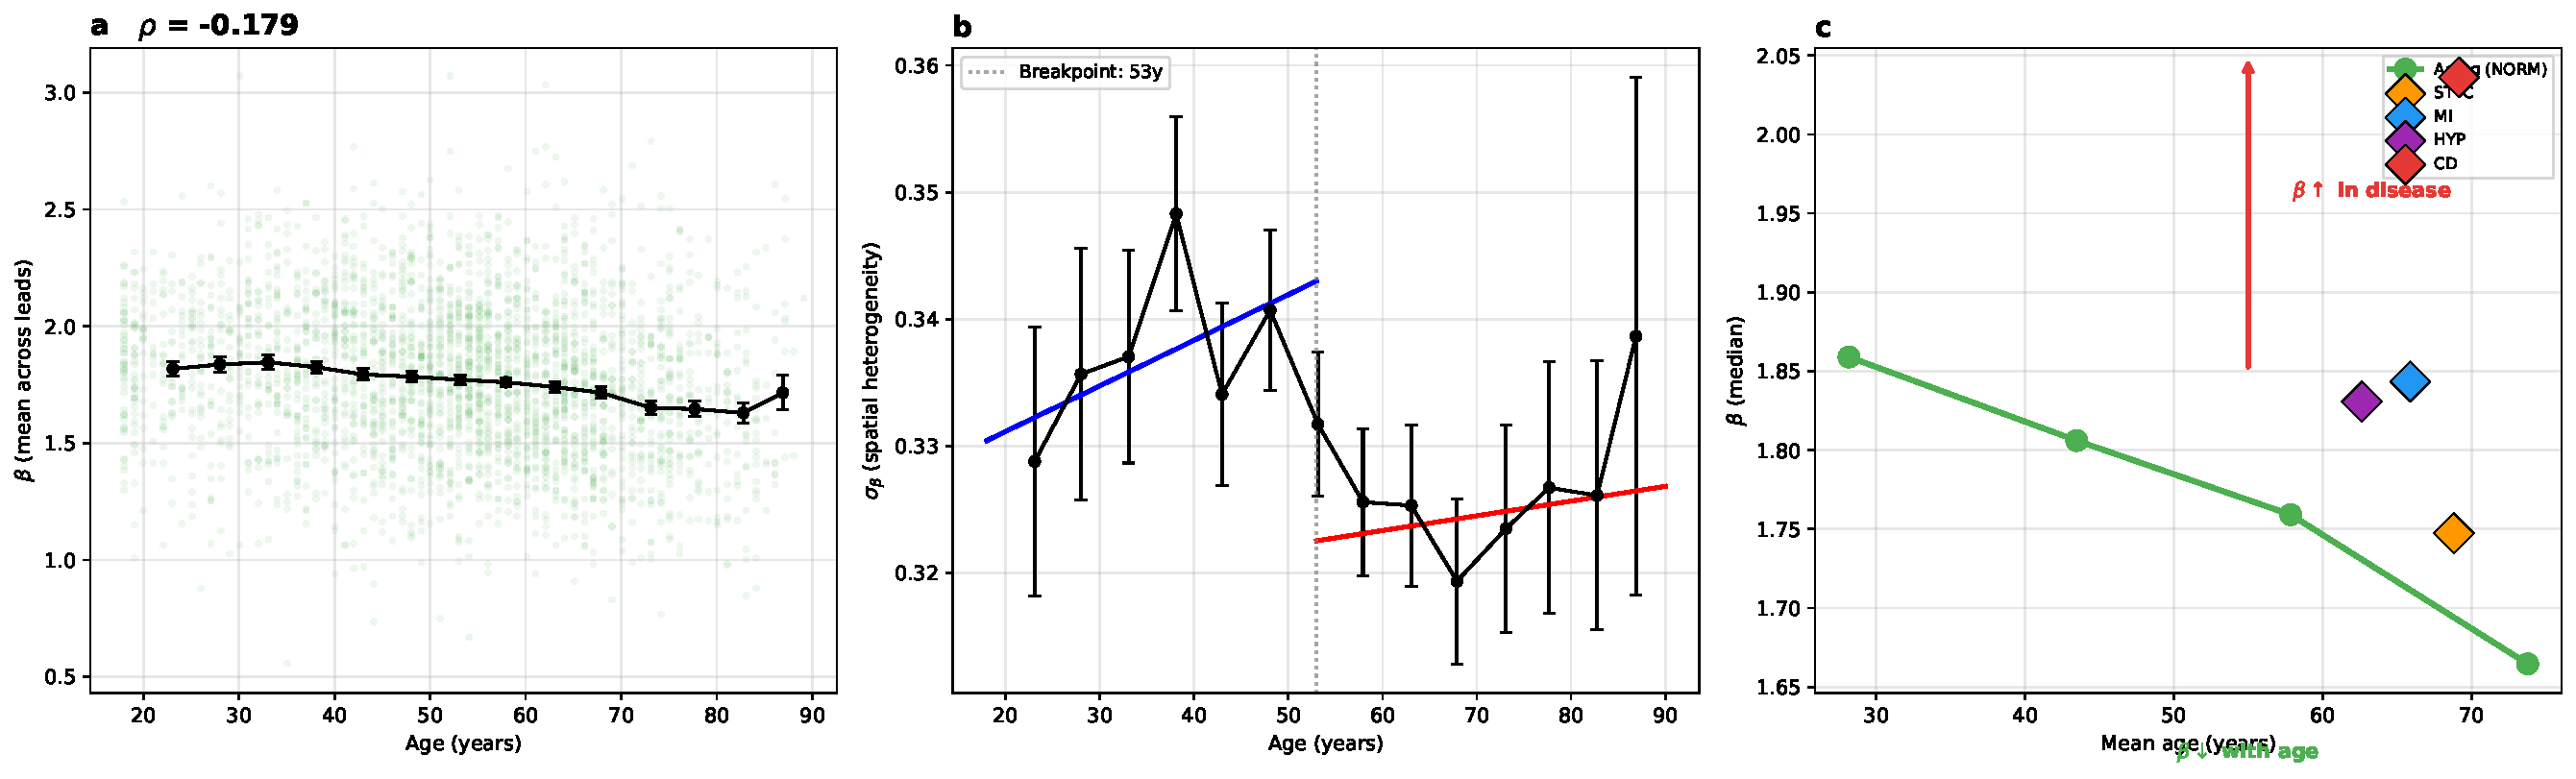
\includegraphics[width=\textwidth]{figures/fig3_aging_bifurcation.pdf}
\caption{\textbf{The aging bifurcation.} (a)~$\beta_\text{mean}$ vs.\ age in 8,940 healthy recordings ($\rho = -0.179$). (b)~Segmented regression of $\sigma_\beta$ with breakpoint at age 53. (c)~Bifurcation diagram: aging ($\beta \downarrow$) vs.\ pathology ($\beta \uparrow$) from the healthy operating point.}
\label{fig:aging}
\end{figure}

\subsection{Subclinical Detection}
Among NORM recordings, 179 had no conduction findings and 328 had subclinical findings. A classifier achieved AUC $= 0.754$ (Figure~\ref{fig:subclinical}c). The strongest feature was $\beta_\text{anterior}$ (Cohen's $d = -0.551$; Figure~\ref{fig:subclinical}b), with subclinical recordings showing \textit{lower} $\beta$---inverted relative to overt CD. Three regimes form a continuum: subclinical fragmentation ($\beta \downarrow$), normal ($\beta \approx 1.76$), overt blockade ($\beta \uparrow$).

\begin{figure}[H]
\centering
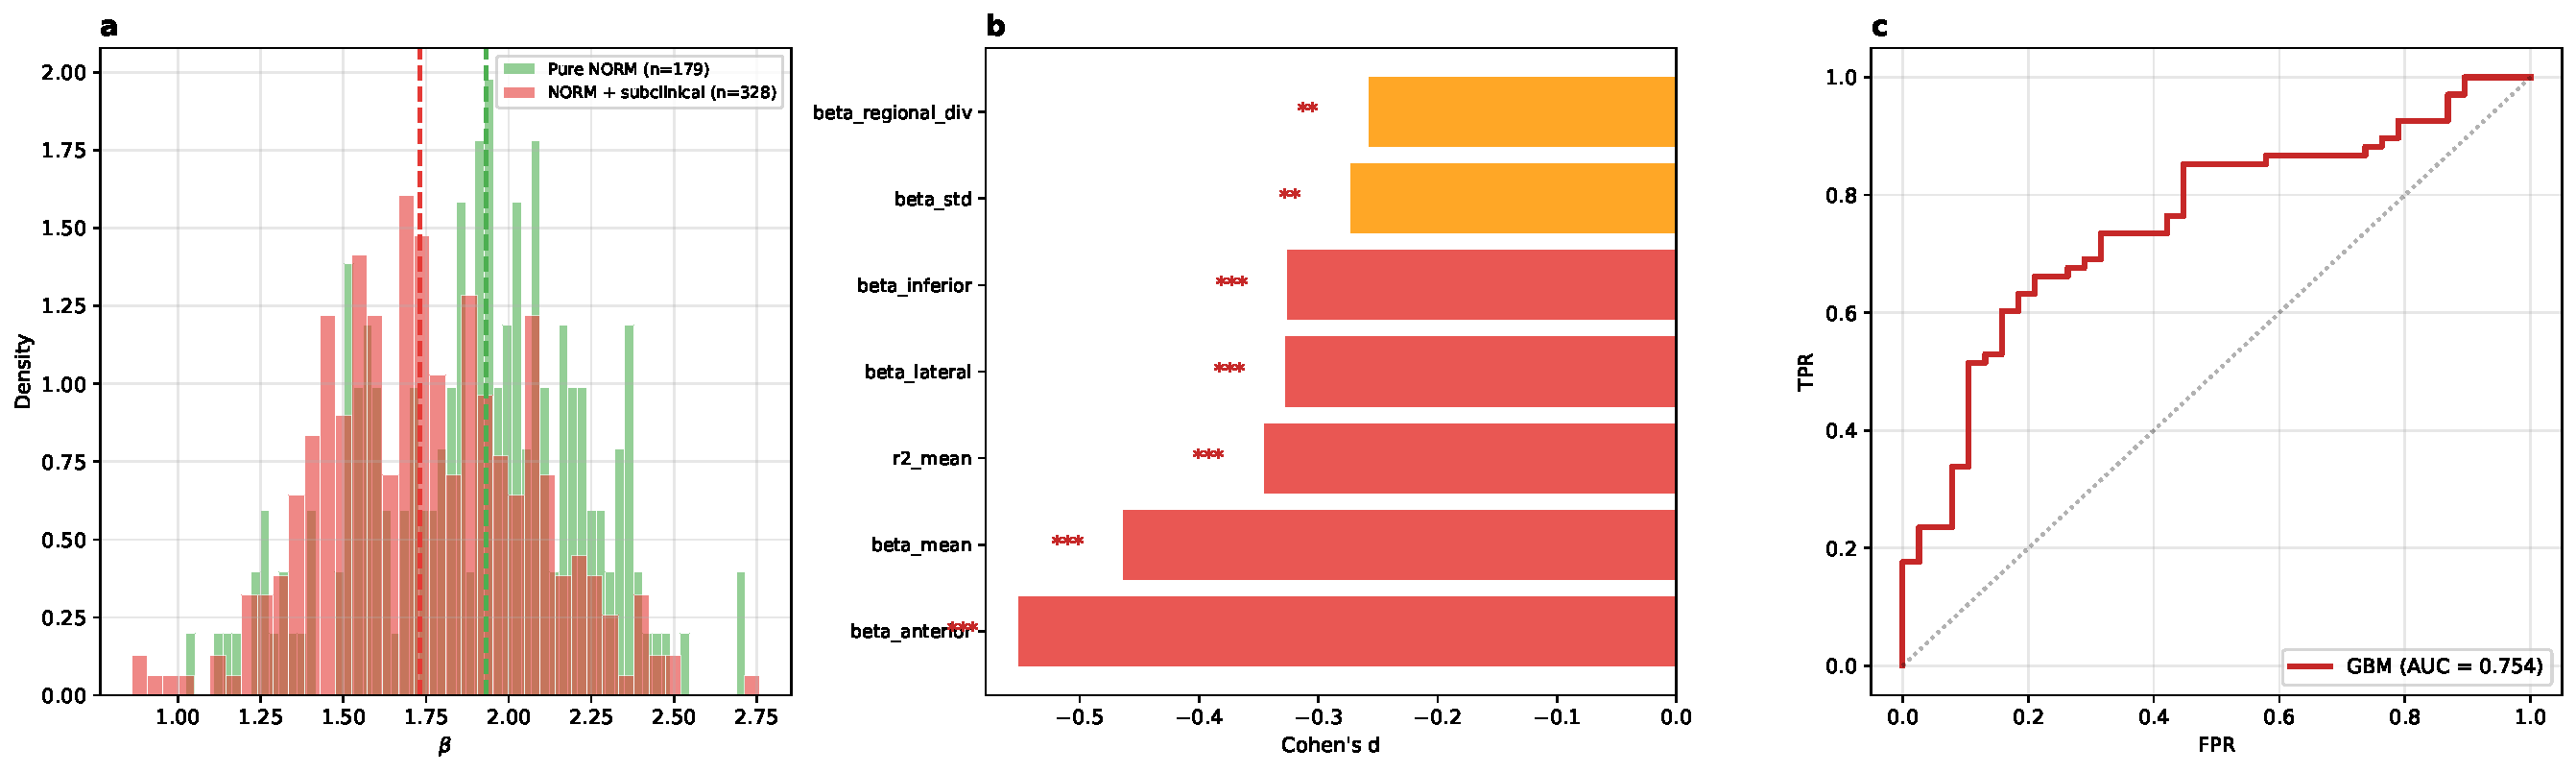
\includegraphics[width=\textwidth]{figures/fig4_subclinical.pdf}
\caption{\textbf{Subclinical detection.} (a)~$\beta_\text{mean}$ distributions: pure NORM vs.\ NORM with subclinical conduction findings. (b)~Cohen's $d$ effect sizes by feature. (c)~ROC: pure NORM vs.\ subclinical (AUC $= 0.754$).}
\label{fig:subclinical}
\end{figure}

\subsection{External Validation Across Three Continents}
We applied the identical IRASA pipeline to two independent external datasets (Figure~\ref{fig:validation}, Table~\ref{tab:validation}).
\begin{table}[H]
\centering
\caption{Cross-population replication of CLBBB vs.\ CRBBB classification.}
\label{tab:validation}
\begin{tabular}{lllrrrrr}
\toprule
Dataset & Country & Equipment & $N$ & CLBBB & CRBBB & $\beta_\text{NORM}$ & AUC \\
\midrule
PTB-XL & Germany & Schiller & 21,799 & 536 & 537 & 1.76 & 0.982 \\
Chapman & China & GE MUSE & 45,152 & 213 & 1,096 & 1.52 & 0.982 \\
CODE-15\% & Brazil & TEB & 345,779 & 414 & 557 & 2.75 & 0.979 \\
\bottomrule
\end{tabular}
\end{table}
The absolute value of $\beta_\text{NORM}$ varied substantially (1.52--2.75), reflecting equipment differences. However, the CLBBB vs.\ CRBBB AUC was virtually identical (0.982, 0.982, 0.979), demonstrating that the \textit{relative geometry} of the twelve-lead $\beta$-vector is invariant to equipment and population.
Spatial fingerprints replicated across all three datasets. The aging trajectory did not replicate externally ($\rho = +0.12$ in Chapman, $\rho = 0.005$ in CODE), likely reflecting absence of curated healthy cohorts and large equipment-related $\beta$-offsets.

\begin{figure}[H]
\centering
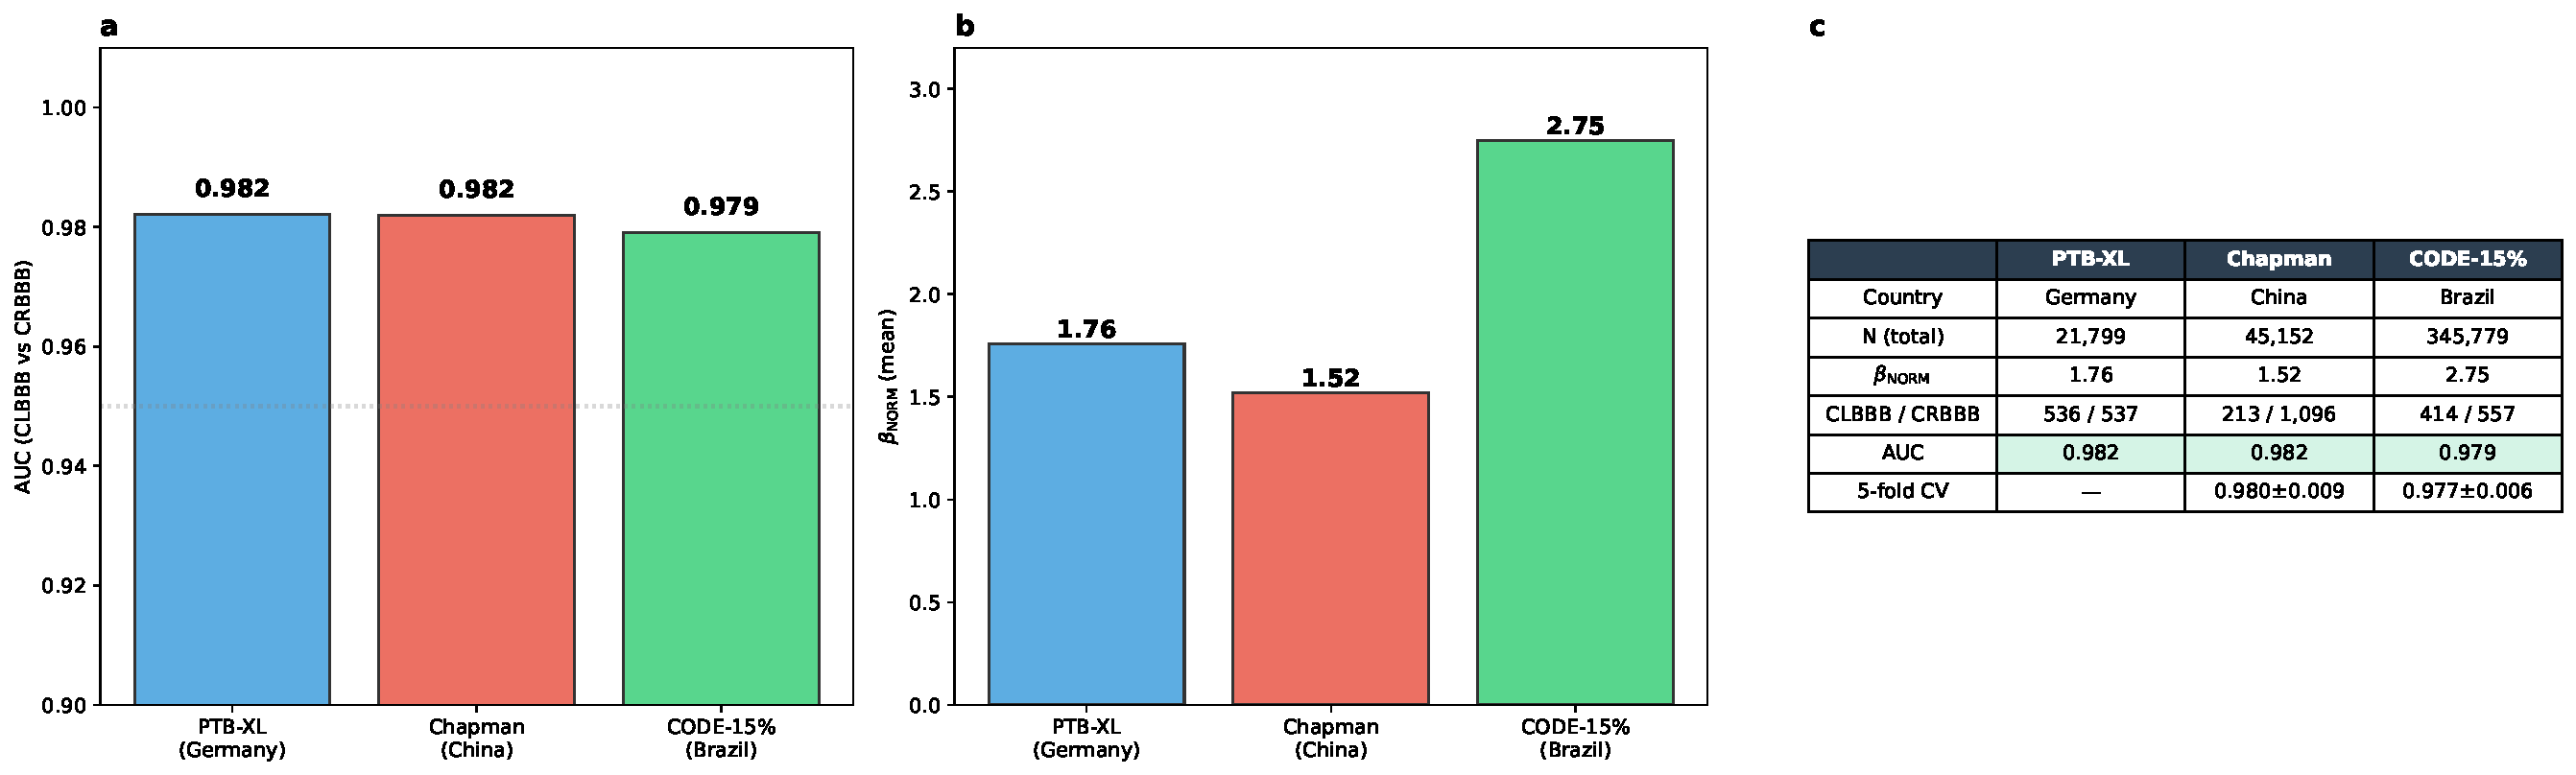
\includegraphics[width=\textwidth]{figures/fig5_external_validation.pdf}
\caption{\textbf{External validation across three continents.} (a)~CLBBB vs.\ CRBBB AUC across datasets. (b)~$\beta_\text{NORM}$ varies by equipment but the classification geometry is invariant. (c)~Cross-dataset summary.}
\label{fig:validation}
\end{figure}

\subsection{Mortality Analysis}
In CODE-15\% ($n = 23{,}833$), higher $\beta_\text{mean}$ was associated with mortality in unadjusted analysis (HR $= 1.79$, 95\% CI 1.48--2.18, $p = 4.2 \times 10^{-9}$). After adjustment for age and sex, the association attenuated (HR $= 1.23$, $p = 0.019$). After full adjustment including diagnostic labels, the association was abolished (HR $= 1.02$, $p = 0.83$). $\beta$ is a diagnostic marker, not an independent prognostic biomarker.
% ================================================================
% 4. DISCUSSION
% ================================================================
\section{Discussion}
\subsection{The Spectral Exponent as a Window onto Cardiac Electrophysiology}
We have shown that a single physics-based parameter---the spectral exponent $\beta$ of the aperiodic ECG component---carries diagnostic information across the full clinical spectrum, from subclinical conduction abnormalities through healthy aging to overt bundle branch block. The key insight is not that $\beta$ is a superior classifier, but that $\beta$ distills a specific physical property: the balance between organized and disorganized broadband activity. This interpretability is the main advantage over black-box approaches.
\subsection{Three Regimes of Cardiac Electrical Complexity}
Our results organize into three regimes. In the \textit{subclinical regime}, incomplete conduction disturbances fragment the wavefront without a dominant alternative pathway---more high-frequency fluctuation, lower $\beta$. In the \textit{normal regime}, coordinated wavefronts yield $\beta \approx 1.76$. In the \textit{overt blockade regime}, a major pathway is interrupted, forcing slow conduction through poorly coupled myocardium---steeper spectrum, higher $\beta$.
Healthy aging follows the trajectory toward the subclinical regime, reflecting diffuse interstitial fibrosis and gap junction remodeling \citep{deJong2011, Jansen2010}. The breakpoint near age 53 coincides approximately with the onset of accelerated age-related ventricular remodeling \citep{Cheng2009}.
\subsection{Cross-Population Invariance: Spectral Anatomy as a Physical Constant}
The near-identical CLBBB vs.\ CRBBB AUC across three datasets (0.982, 0.982, 0.979)---spanning three continents, recording systems, and populations---is the central result. This invariance persists despite factor-of-two variation in absolute $\beta$-values, demonstrating that absolute $\beta$ is equipment-dependent but the \textit{relative geometry} of the $\beta$-vector is determined by anatomy.
The physical explanation is straightforward: the left bundle passes through the interventricular septum beneath V1--V4 in every human heart, and the right bundle passes close to V1. These anatomical relationships are invariant. The twelve-lead $\beta$-vector is a low-dimensional spectral image of conduction system integrity.
\subsection{Comparison with Prior Work}
The HRV literature has extensively characterized $1/f$ scaling in RR-interval fluctuations \citep{Peng1995, Ivanov1999, Goldberger2002}. Our work extends the fractal dynamics framework to the ECG waveform itself---a fundamentally different signal reflecting collective myocardial depolarization rather than autonomic modulation. The healthy $\beta \approx 1.76$ (near Brownian noise) contrasts with healthy HRV $\alpha \approx 1.0$ (pink noise), consistent with different physiological mechanisms.
\citet{Schmidt2025} showed ECG spectral slope flattens with age using IRASA on $\sim$2,300 recordings. We confirm and extend this on a larger dataset and additionally demonstrate diagnostic specificity, the aging-pathology bifurcation, and cross-population invariance. \citet{Contoyiannis2021} found MI patients are ``far from criticality''---conceptually aligned with our observation. \citet{George2025} achieved AUC $= 0.90$ on PTB-XL with Higuchi fractal dimension; our approach provides the spatial anatomical mapping as central contribution.
\subsection{Limitations and Calibration of Claims}
\textbf{Replicated across three datasets:} diagnostic $\beta$-landscape, spatial fingerprints, CLBBB vs.\ CRBBB classification, diagnostic ordering. These are our strongest claims.
\textbf{PTB-XL only:} aging bifurcation, beat-to-beat variability, subclinical detection. The aging trajectory did not replicate externally ($\rho = +0.12$ in Chapman, $\rho = 0.005$ in CODE-15\%---opposite or null). This is likely because (i)~equipment-related $\beta$-offsets ($\beta_\text{NORM}$ ranges from 1.52 to 2.75) dominate the subtle aging signal ($\Delta\beta \approx 0.1$ per decade), and (ii)~external datasets lack curated healthy cohorts with confirmed absence of pathology. The aging findings should therefore be considered a PTB-XL observation requiring independent validation, not a confirmed cross-population result.
\textbf{Honest null results:} $\beta$ does not independently predict mortality (adjusted HR $= 1.02$). Absolute $\beta$ is equipment-dependent. $\beta$ does not correlate with age in uncurated populations.
\textbf{Subclinical detection} is hypothesis-generating: AUC $= 0.754$ in a single dataset with a small sample ($n = 507$). External validation on datasets with annotated subclinical conduction findings is needed before clinical conclusions can be drawn.
\textbf{Relationship to standard morphological features:} $\beta$ may partially reflect QRS duration, since bundle branch block widens the QRS complex and steepens the spectrum. Future work should quantify the incremental information in $\beta$ beyond standard ECG intervals (QRS duration, QT interval, PR interval) to establish whether $\beta$ captures conduction properties not already encoded in morphological measurements.
Additional limitations: (1)~ten-second duration; (2)~cross-sectional design; (3)~no medication data; (4)~inability to separate autonomic from intrinsic myocardial effects; (5)~wearable utility (reduced leads) untested.
\subsection{Clinical Implications and Future Directions}
The cross-equipment invariance suggests $\beta$-based characterization could be deployed across heterogeneous environments without device-specific recalibration. However, $\beta$ does not replace existing methods. Its value lies in: (1)~interpretability; (2)~equipment-invariance of relative patterns; and (3)~computability without waveform delineation.
Whether these translate to clinical utility in wearable screening, longitudinal monitoring, or telemedicine remains to be determined. Priorities include single-lead validation, longitudinal $\beta$-tracking, and investigation of the molecular substrate using single-cell transcriptomic data from aging hearts \citep{TabulaMuris2020}.
% ================================================================
% DATA AND CODE AVAILABILITY
% ================================================================
\section*{Ethics Statement}
This study exclusively uses publicly available, de-identified datasets previously approved for research use by institutional review boards at the originating institutions: PTB-XL (Physikalisch-Technische Bundesanstalt, Berlin), Chapman-Shaoxing (Shaoxing People's Hospital), and CODE-15\% (Telehealth Network of Minas Gerais, approved by the Research Ethics Committee of the Universidade Federal de Minas Gerais). No additional ethical approval was required for this secondary analysis of de-identified data.
\section*{Author Contributions}
T.S.\ conceived the study, designed and performed all analyses, generated all figures, and wrote the manuscript.
\section*{Data and Code Availability}
All data are publicly available: PTB-XL (\url{https://physionet.org/content/ptb-xl/}), Chapman-Shaoxing (\url{https://physionet.org/content/ecg-arrhythmia/}), CODE-15\% (\url{https://zenodo.org/records/4916206}). Analysis code is available as a Kaggle notebook: [TODO: insert Kaggle URL] and on GitHub: [TODO: insert GitHub URL].
\section*{Declaration of Interests}
The author has no financial or non-financial competing interests to declare.
\section*{Funding}
No external funding was received for this work.
% ================================================================
% REFERENCES
% ================================================================
\bibliographystyle{unsrtnat}
\begin{thebibliography}{99}
\bibitem[Babayan et~al.(2019)]{Babayan2019}
Babayan A, et~al.
\newblock A mind-brain-body dataset of MRI, EEG, cognition, emotion, and peripheral physiology in young and old adults.
\newblock \textit{Scientific Data}. 2019;6:180308.
\bibitem[Cheng et~al.(2009)]{Cheng2009}
Cheng S, Xanthakis V, Sullivan LM, et~al.
\newblock Correlates of echocardiographic indices of cardiac remodeling over the adult life course.
\newblock \textit{Circulation}. 2009;119:2563--2571.
\bibitem[Contoyiannis et~al.(2021)]{Contoyiannis2021}
Contoyiannis Y, Stavrinides SG, Hanias MP, et~al.
\newblock Can high-frequency ECG fluctuations differentiate between healthy and myocardial infarction cases?
\newblock \textit{Results in Physics}. 2021;25:104169.
\bibitem[de~Jong et~al.(2011)]{deJong2011}
de~Jong S, van~Veen TAB, van~Rijen HVM, de~Bakker JMT.
\newblock Fibrosis and cardiac arrhythmias.
\newblock \textit{J Cardiovasc Pharmacol}. 2011;57(6):630--638.
\bibitem[Gao et~al.(2017)]{Gao2017}
Gao R, Peterson EJ, Voytek B.
\newblock Inferring synaptic excitation/inhibition balance from field potentials.
\newblock \textit{NeuroImage}. 2017;158:70--78.
\bibitem[George et~al.(2025)]{George2025}
George T, et~al.
\newblock Exploring complexity changes in diseased ECG signals for enhanced classification.
\newblock \textit{arXiv:2510.17810}. 2025.
\bibitem[Goldberger et~al.(2002)]{Goldberger2002}
Goldberger AL, Amaral LAN, Hausdorff JM, et~al.
\newblock Fractal dynamics in physiology: alterations with disease and aging.
\newblock \textit{Proc Natl Acad Sci USA}. 2002;99(suppl 1):2466--2472.
\bibitem[Ivanov et~al.(1999)]{Ivanov1999}
Ivanov PCh, Amaral LAN, Goldberger AL, et~al.
\newblock Multifractality in human heartbeat dynamics.
\newblock \textit{Nature}. 1999;399:461--465.
\bibitem[Jansen et~al.(2010)]{Jansen2010}
Jansen JA, van~Veen TAB, de~Bakker JMT, van~Rijen HVM.
\newblock Cardiac connexins and impulse propagation.
\newblock \textit{J Mol Cell Cardiol}. 2010;48(1):76--82.
\bibitem[Lendner et~al.(2020)]{Lendner2020}
Lendner JD, Helfrich RF, Mander BA, et~al.
\newblock An electrophysiological marker of arousal level in humans.
\newblock \textit{eLife}. 2020;9:e55092.
\bibitem[Lipsitz \& Goldberger(1992)]{Lipsitz1992}
Lipsitz LA, Goldberger AL.
\newblock Loss of `complexity' and aging.
\newblock \textit{JAMA}. 1992;267(13):1806--1809.
\bibitem[Peng et~al.(1995)]{Peng1995}
Peng C-K, Havlin S, Stanley HE, Goldberger AL.
\newblock Quantification of scaling exponents and crossover phenomena in nonstationary heartbeat time series.
\newblock \textit{Chaos}. 1995;5(1):82--87.
\bibitem[Ribeiro et~al.(2020)]{Ribeiro2020}
Ribeiro AH, Ribeiro MH, Paix\~{a}o GMM, et~al.
\newblock Automatic diagnosis of the 12-lead ECG using a deep neural network.
\newblock \textit{Nat Commun}. 2020;11:1760.
\bibitem[Schmidt et~al.(2025)]{Schmidt2025}
Schmidt H, Bielczyk NZ, Krasnozhon A, et~al.
\newblock Age-related changes in ``cortical'' 1/f dynamics are linked to cardiac activity.
\newblock \textit{eLife}. 2025;13:RP102750.
\bibitem[Shekatkar et~al.(2017)]{Shekatkar2017}
Shekatkar SM, Kotriwar Y, Harikrishnan KP, Ambika G.
\newblock Detecting abnormality in heart dynamics from multifractal analysis of ECG signals.
\newblock \textit{Sci Rep}. 2017;7:15127.
\bibitem[Strodthoff et~al.(2021)]{Strodthoff2021}
Strodthoff N, Wagner P, Schaeffter T, Samek W.
\newblock Deep learning for ECG analysis: benchmarks and insights from PTB-XL.
\newblock \textit{IEEE J Biomed Health Inform}. 2021;25(5):1519--1528.
\bibitem[Tabula Muris Consortium(2020)]{TabulaMuris2020}
Tabula Muris Consortium.
\newblock A single-cell transcriptomic atlas characterizes ageing tissues in the mouse.
\newblock \textit{Nature}. 2020;583:590--595.
\bibitem[Voytek et~al.(2015)]{Voytek2015}
Voytek B, Kramer MA, Case J, et~al.
\newblock Age-related changes in 1/f neural electrophysiological noise.
\newblock \textit{J Neurosci}. 2015;35(38):13257--13265.
\bibitem[Wagner et~al.(2020)]{Wagner2020}
Wagner P, Strodthoff N, Bousseljot R-D, et~al.
\newblock PTB-XL, a large publicly available electrocardiography dataset.
\newblock \textit{Sci Data}. 2020;7:154.
\bibitem[Wen \& Liu(2016)]{Wen2016}
Wen H, Liu Z.
\newblock Separating fractal and oscillatory components in the power spectrum.
\newblock \textit{Brain Topogr}. 2016;29(1):13--26.
\bibitem[Yang et~al.(2020)]{Yang2020}
Yang J, Ning X, He A.
\newblock Identification of healthy and pathological heartbeat dynamics based on ECG-waveform using multifractal spectrum.
\newblock \textit{Physica A}. 2020;559:125021.
\bibitem[Zheng et~al.(2020)]{Zheng2020}
Zheng J, Zhang J, Danioko S, et~al.
\newblock A 12-lead electrocardiogram database for arrhythmia research covering more than 10,000 patients.
\newblock \textit{Sci Data}. 2020;7:48.
\end{thebibliography}
% ================================================================
% SUPPLEMENTARY
% ================================================================
\newpage
\section*{Supplementary Information}

\subsection*{Table S1. Pairwise superclass comparisons}
\begin{table}[H]
\centering
\small
\begin{tabular}{lrrrrrc}
\toprule
Comparison & $n_1$ & $n_2$ & $\bar{\beta}_1$ & $\bar{\beta}_2$ & Cohen's $d$ & $p$ (Bonferroni) \\
\midrule
NORM vs CD   & 9,068 & 1,708 & 1.760 & 2.151 & 0.989 & $< 10^{-120}$ \\
STTC vs CD   & 2,400 & 1,708 & 1.768 & 2.151 & 0.760 & $< 10^{-80}$ \\
MI vs CD     & 2,532 & 1,708 & 1.859 & 2.151 & 0.577 & $< 10^{-40}$ \\
HYP vs CD    & 534   & 1,708 & 1.859 & 2.151 & 0.501 & $< 10^{-16}$ \\
NORM vs HYP  & 9,068 & 534   & 1.760 & 1.859 & 0.293 & $3.0 \times 10^{-7}$ \\
NORM vs MI   & 9,068 & 2,532 & 1.760 & 1.859 & 0.281 & $< 10^{-23}$ \\
STTC vs HYP  & 2,400 & 534   & 1.768 & 1.859 & 0.231 & $6.6 \times 10^{-6}$ \\
MI vs STTC   & 2,532 & 2,400 & 1.859 & 1.768 & $-0.227$ & $< 10^{-13}$ \\
NORM vs STTC & 9,068 & 2,400 & 1.760 & 1.768 & 0.023 & 1.0 (n.s.) \\
MI vs HYP    & 2,532 & 534   & 1.859 & 1.859 & 0.002 & 1.0 (n.s.) \\
\bottomrule
\end{tabular}
\caption*{Single-label assignments used. $p$-values Bonferroni-corrected for 10 comparisons.}
\end{table}

\subsection*{Table S2. Per-subtype CD metrics}
\begin{table}[H]
\centering
\begin{tabular}{lrrrc}
\toprule
Subtype & $n$ & $\beta_\text{mean} \pm$ SD & Cohen's $d$ vs NORM \\
\midrule
CLBBB & 536 & $2.923 \pm 0.394$ & 3.438 \\
CRBBB & 537 & $2.142 \pm 0.490$ & 1.107 \\
IVCD  & 780 & $2.131 \pm 0.482$ & 1.064 \\
LAFB  & 1,604 & $2.070 \pm 0.508$ & 0.848 \\
1AVB  & 779 & $2.062 \pm 0.554$ & 0.847 \\
IRBBB & 1,102 & $1.771 \pm 0.377$ & 0.033 \\
\bottomrule
\end{tabular}
\caption*{Sorted by descending Cohen's $d$. Counts use $\geq 80\%$ annotator confidence threshold.}
\end{table}

\subsection*{Table S3. Segmented regression parameters}
\begin{table}[H]
\centering
\begin{tabular}{lrrrrr}
\toprule
Metric & Breakpoint & Slope (left) & Slope (right) & $F$ & $p$ \\
\midrule
$\beta_\text{mean}$ & 32 y & $+0.0046$/y & $-0.0039$/y & 13.5 & $1.4 \times 10^{-6}$ \\
$\sigma_\beta$       & 53 y & $+0.00036$/y & $+0.00012$/y & 17.8 & $1.9 \times 10^{-8}$ \\
\bottomrule
\end{tabular}
\caption*{Fitted on $n = 8{,}940$ NORM recordings (age 18--95). $\sigma_\beta$ shows acceleration of spatial heterogeneity after age 53.}
\end{table}

\subsection*{Table S4. Demographics by diagnostic superclass}
\begin{table}[H]
\centering
\begin{tabular}{lrrrr}
\toprule
Superclass & $n$ & Male (\%) & Age (mean $\pm$ SD) \\
\midrule
NORM & 9,514 & 46.1 & $52.1 \pm 17.2$ \\
MI   & 5,469 & 62.3 & $66.3 \pm 12.5$ \\
STTC & 5,235 & 49.0 & $66.3 \pm 13.5$ \\
CD   & 4,898 & 61.2 & $65.3 \pm 15.0$ \\
HYP  & 2,649 & 57.4 & $65.9 \pm 13.9$ \\
\midrule
Total & 21,799 & 52.1 & $59.5 \pm 16.8$ \\
\bottomrule
\end{tabular}
\caption*{Multi-label counts (recordings may appear in multiple superclasses). One age outlier (300 y) excluded from age statistics.}
\end{table}

\subsection*{Figure S1. IRASA fit quality ($R^2$ distribution)}
\begin{figure}[H]
\centering
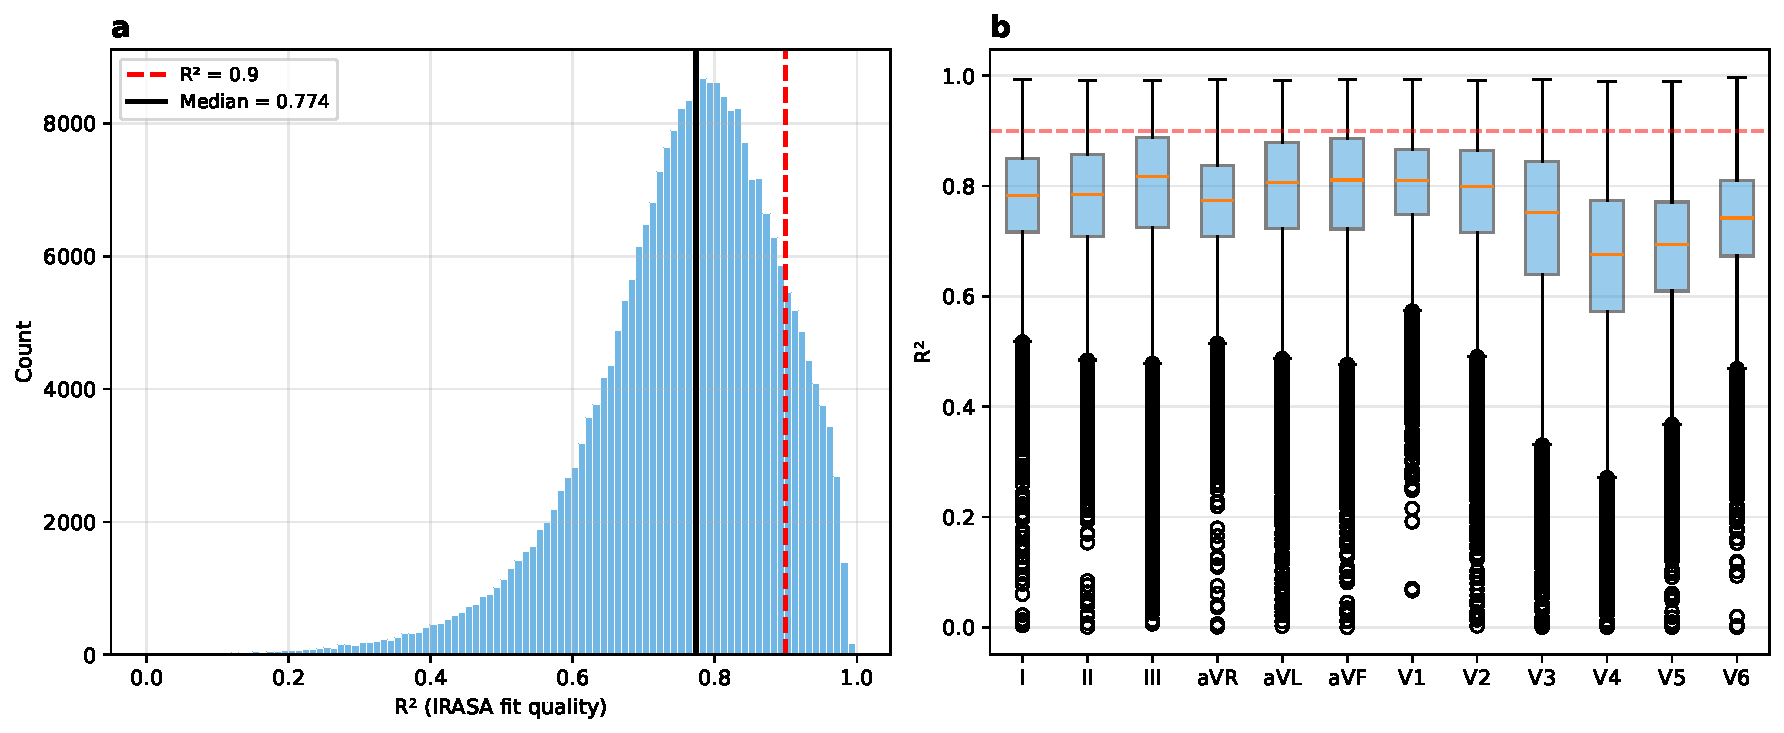
\includegraphics[width=\textwidth]{figures/fig_s1_r2_distribution.pdf}
\caption{(a)~Histogram of $R^2$ values across all leads and recordings (median $= 0.774$). (b)~$R^2$ by lead: precordial leads V1--V2 show highest $R^2$, reflecting stronger $1/f$ structure near the septum.}
\end{figure}

\subsection*{Figure S2. Sensitivity analyses}
\begin{figure}[H]
\centering
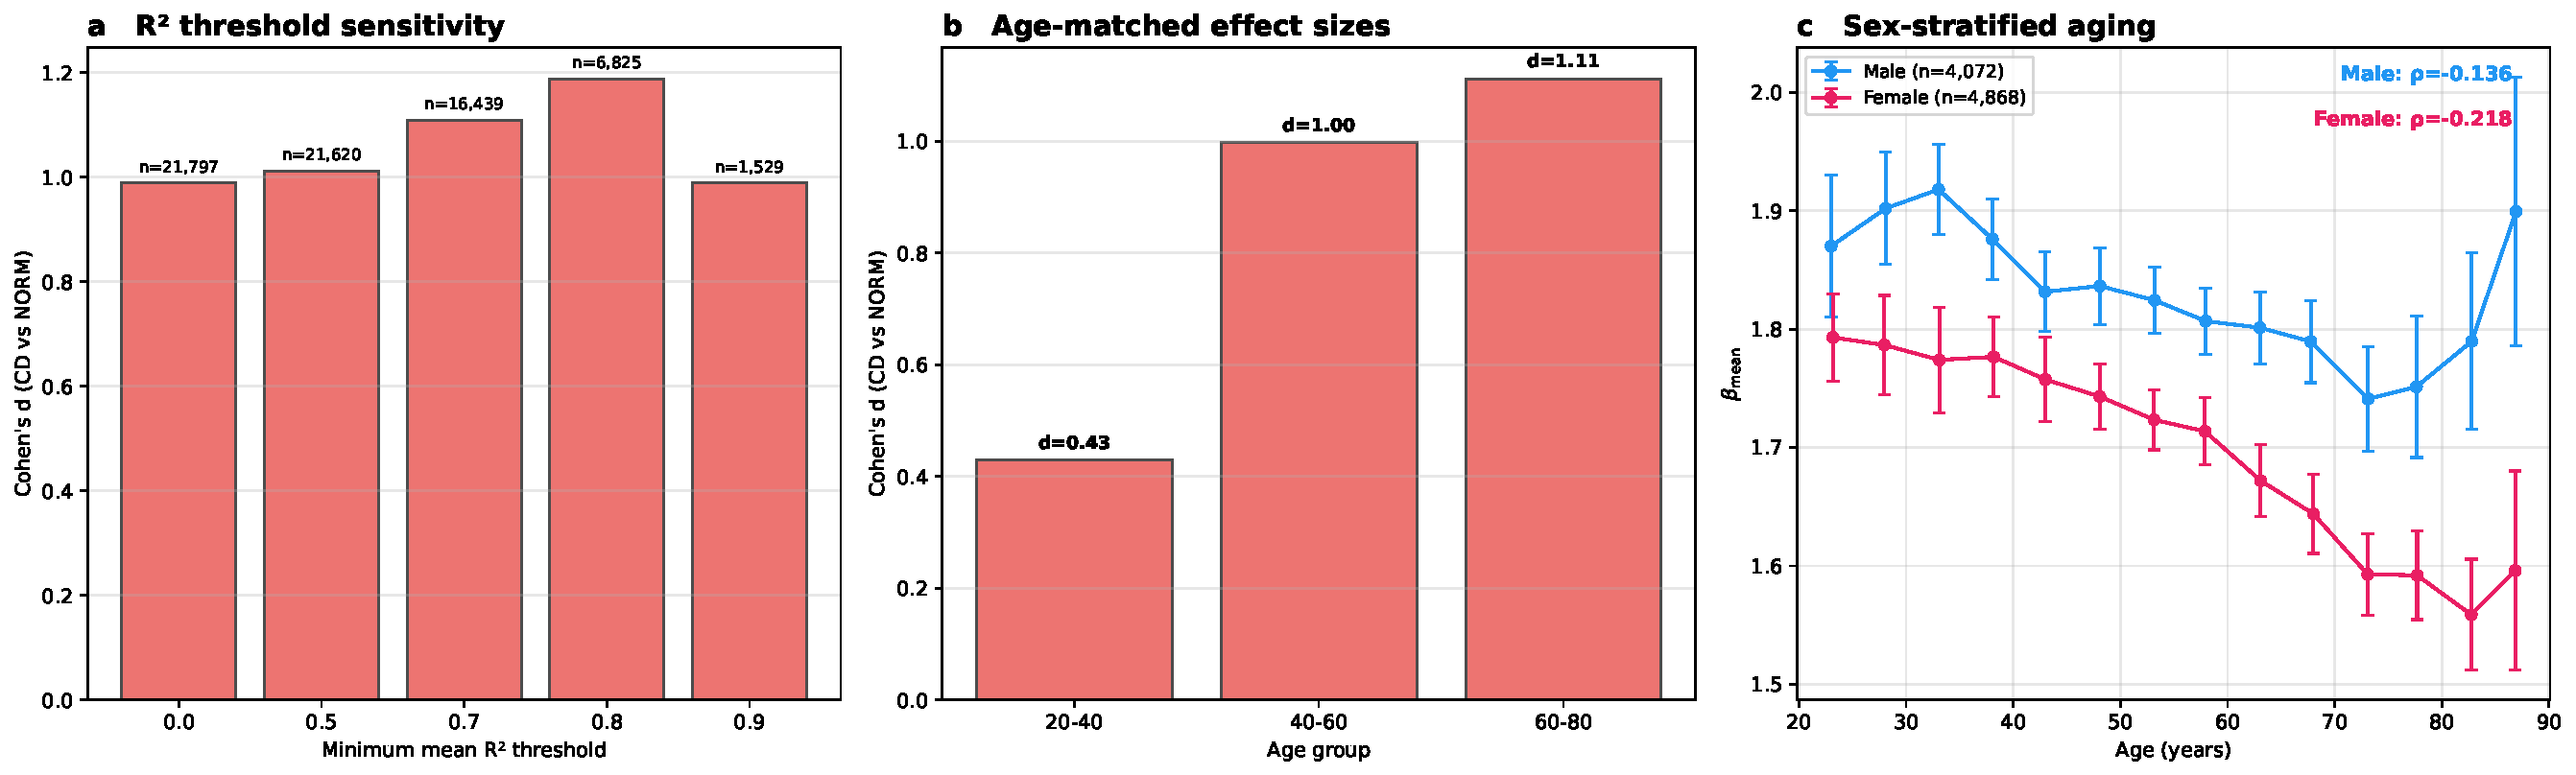
\includegraphics[width=\textwidth]{figures/fig_s2_sensitivity.pdf}
\caption{(a)~CD vs.\ NORM effect size is robust to $R^2$ quality thresholds. (b)~Age-matched subsamples confirm the diagnostic effect is not driven by age confounding. (c)~Sex-stratified aging trajectories: women show steeper decline ($\rho = -0.218$ vs.\ $-0.136$ for men).}
\end{figure}

\end{document}
